\chapter{Design}
\label{Chapter:Design}

This chapter discusses the design considerations taken during the design development of the system. The design stage is very important since it lays down the foundation for the whole system.
Thus a considerable amount of time has been spent in designing the system. \citet[12]{bell2005} states that about 5\% of the total time that takes for the development of a software should be spent for the design state alone. For comparison, the coding process takes about 7\%; Testing takes 8\%. 

The design process has gone through many iterations to ensure the best possible quality of the product. The research presented in chapter \ref{Chapter:Literature-Review} has affected immensely the design, especially section \ref{section:commercial-har-systems}. The design can be split into four main sections, namely Mobile Platform and IDE; Database Design; Architectural design and User Interface (UI).

    \section{Mobile Platform and IDE}
        The first point that was considered in the design process was the \textbf{mobile platform} on which the proposed application will be implemented and distributed. After research on the current market, Google's \textit{Android} was fount to dominate in Europe \citep{williams2016}. Android-based smartphones hold 75.6\% of market share dominating other mobile platforms such as Apple's \textit{iOS} and Microsoft's \textit{Windows Phone}. Thus, Android OS was chosen to form the basis of the proposed mobile application since it will allow the application to be downloaded and used by as many people as possible.
        
        After choosing the mobile platform, one important decision is to choose the development environment or the \textbf{Integrated Development Environment} (\gls{ide}) that will be used to develop the application. That was an easy decision since Android Studio is known to be the official \gls{ide} for Android development \citep{androidstudio2017}.
        
    \section{Architectural design}
    This section discusses the software design choices made during the development of the system. The architectural design is the first stage in the design process of a system. It creates a critical link between the requirements discussed in Chapter \ref{Chapter:Specification} and the research knowledge gained in Chapter \ref{Chapter:Literature-Review}. The end-goal of the architectural design is to discover the major structural components of the system and how they communicate to each other \citep[148]{sommerville2010}. The architectural model of the system can be seen in figure \ref{fig:architectural_design_component_diagram}. The model of the system will be discussed in the following sections.
    
    \begin{figure}[ht]
        \centering
        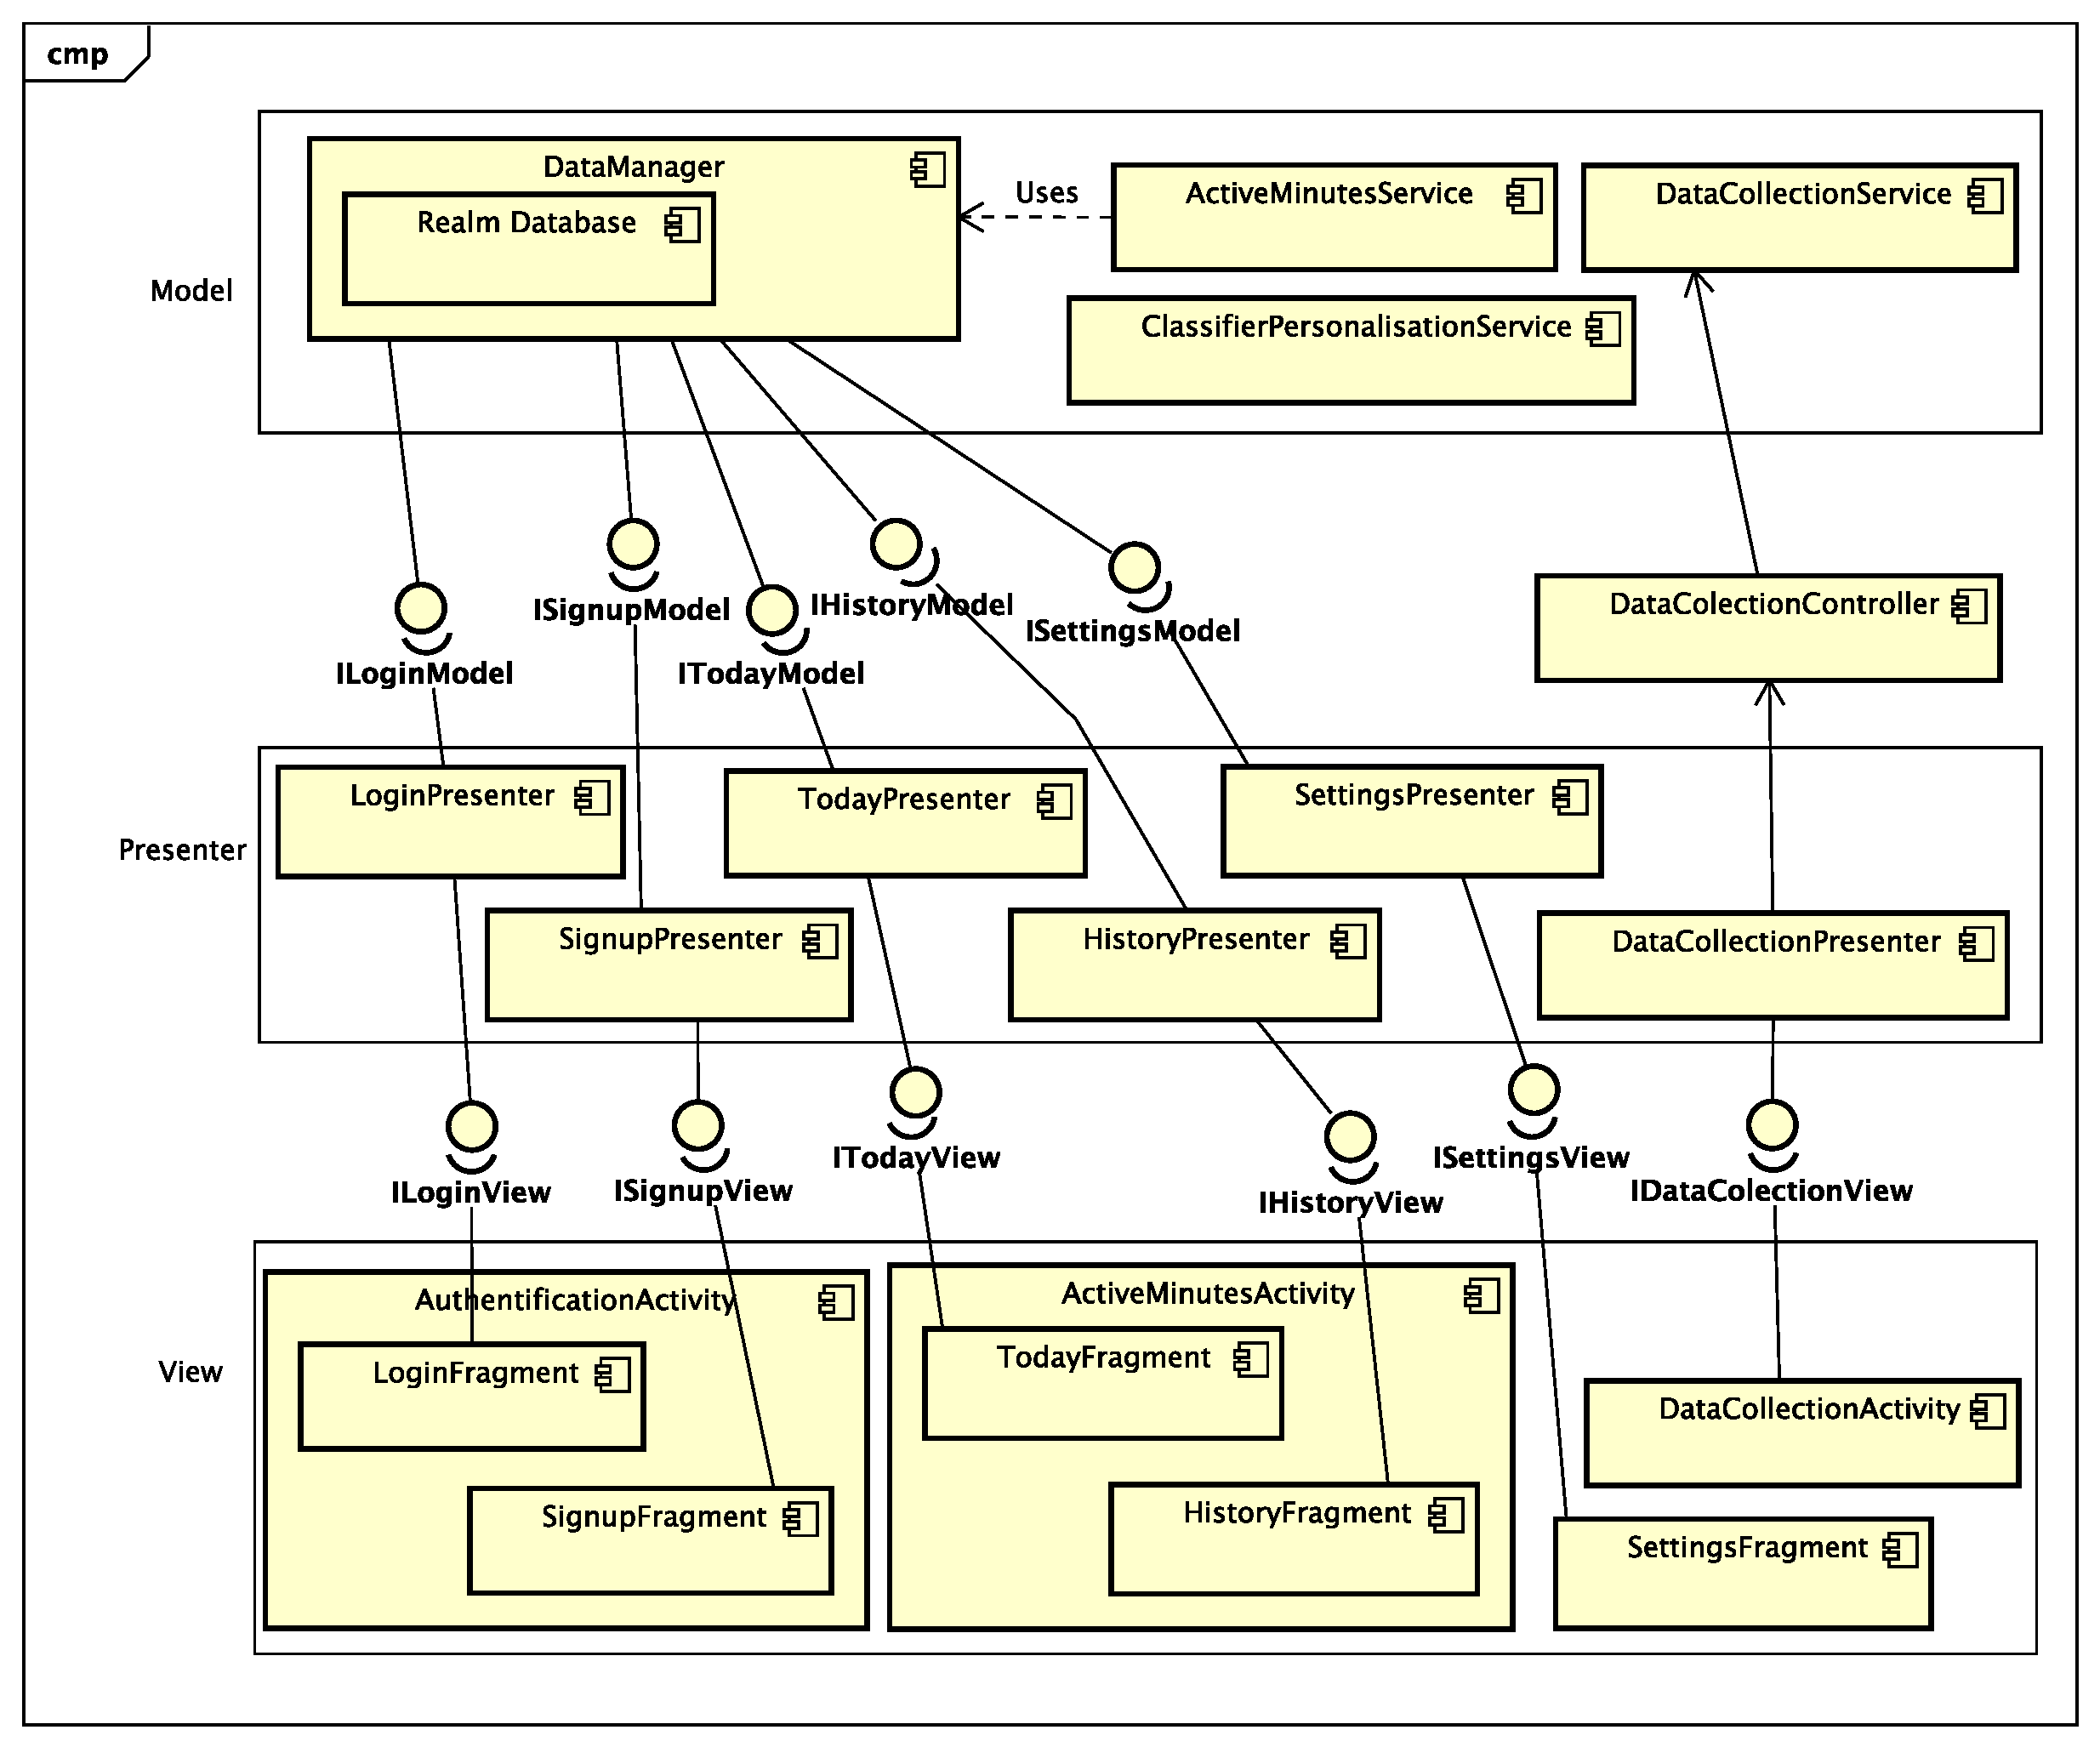
\includegraphics[width=15cm]{active-minutes-service-component-diagram}
        \caption{ \textit{"Active Minutes"} Architectural model}
        \label{fig:architectural_design_component_diagram}
    \end{figure}
    
        \subsection{Architectural pattern}
        Model-View-Presenter or \textbf{MVP} software architectural pattern was chosen to form the base of the proposed mobile system since it provides clean separation of concepts \citep[532]{zhang2010}. For example the \textit{View} represents the \gls{ui} of the application. It contains logic only for receiving user interaction and passing it to the \textit{Presenter}. The\textit{Model} is the data layer. It is responsible for providing and formatting (i.e. applying the business logic) to the date and returning it to the Presenter. The \textit{Presenter} acts as a mediator, it requests data from the \textit{Model} and returns it to update the \textit{View}. Figure \ref{fig:model_view_presenter_design_pattern} shows the interaction flow of the pattern. When the user interacts with the \gls{ui} of mobile application, the View receives the interaction (i.e. button click) and passes that information to the Presenter via Interface (\textit{IView}). The Presenter then invokes the appropriate method of the Model. Next, the Model returns the requested data to the View (via the Presenter). 
        
        The main advantages of using the \gls{mvp} pattern is that it increases the \textbf{testability} of the software via the concept of logic separation. For example, the View is only allowed to have framework specific code (i.e. Android UI components such as Button, ListView); Presenter and Model are comprised of Plain Old Java Objects or \textbf{POJO}. These POJO classes can be thoroughly tested outside the mobile application. In addition, the \gls{mvp} pattern introduces a certain level of abstraction in the architecture of the software (via the use of Interfaces, see figure \ref{fig:architectural_design_component_diagram}). That allows different parts of the software to be developed separately and then integrated into the application.
    
        \begin{figure}[h!]
            \centering
            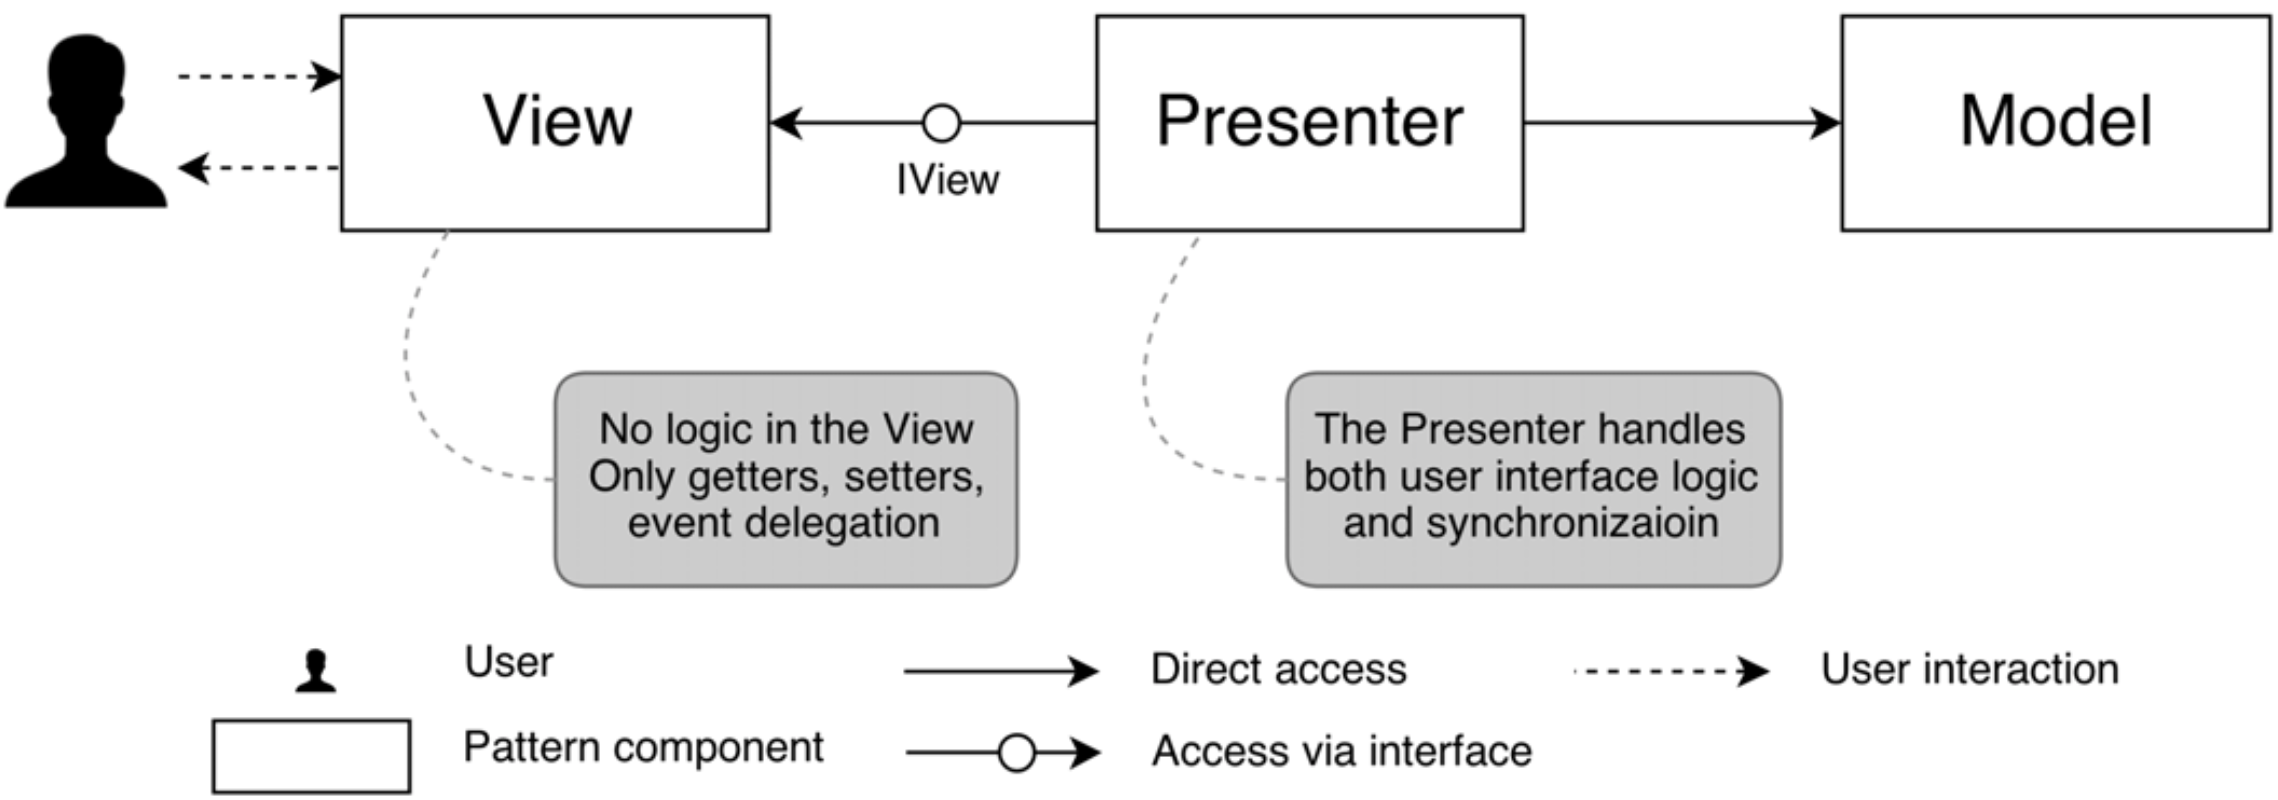
\includegraphics[width=13cm]{model-view-presenter-design-pattern}
            \caption{Model-View-Presenter design pattern \citep[28]{syromiatnikov2014}}
            \label{fig:model_view_presenter_design_pattern}
        \end{figure}
   
    
    
    \section{Database Design}
    This section discuses the design of the database system that will be used to store data of \textit{"Active Minutes"} mobile application. The design of the database can be seen in figure \ref{fig:data_modeling_er_diagram}. It includes the following entities \textbf{User}, \textbf{Activity} and \textbf{Training\_data}. The following sections will explain the responsibilities of each entity (i.e.\ database tables).
        
        \begin{figure}[ht]
            \centering
            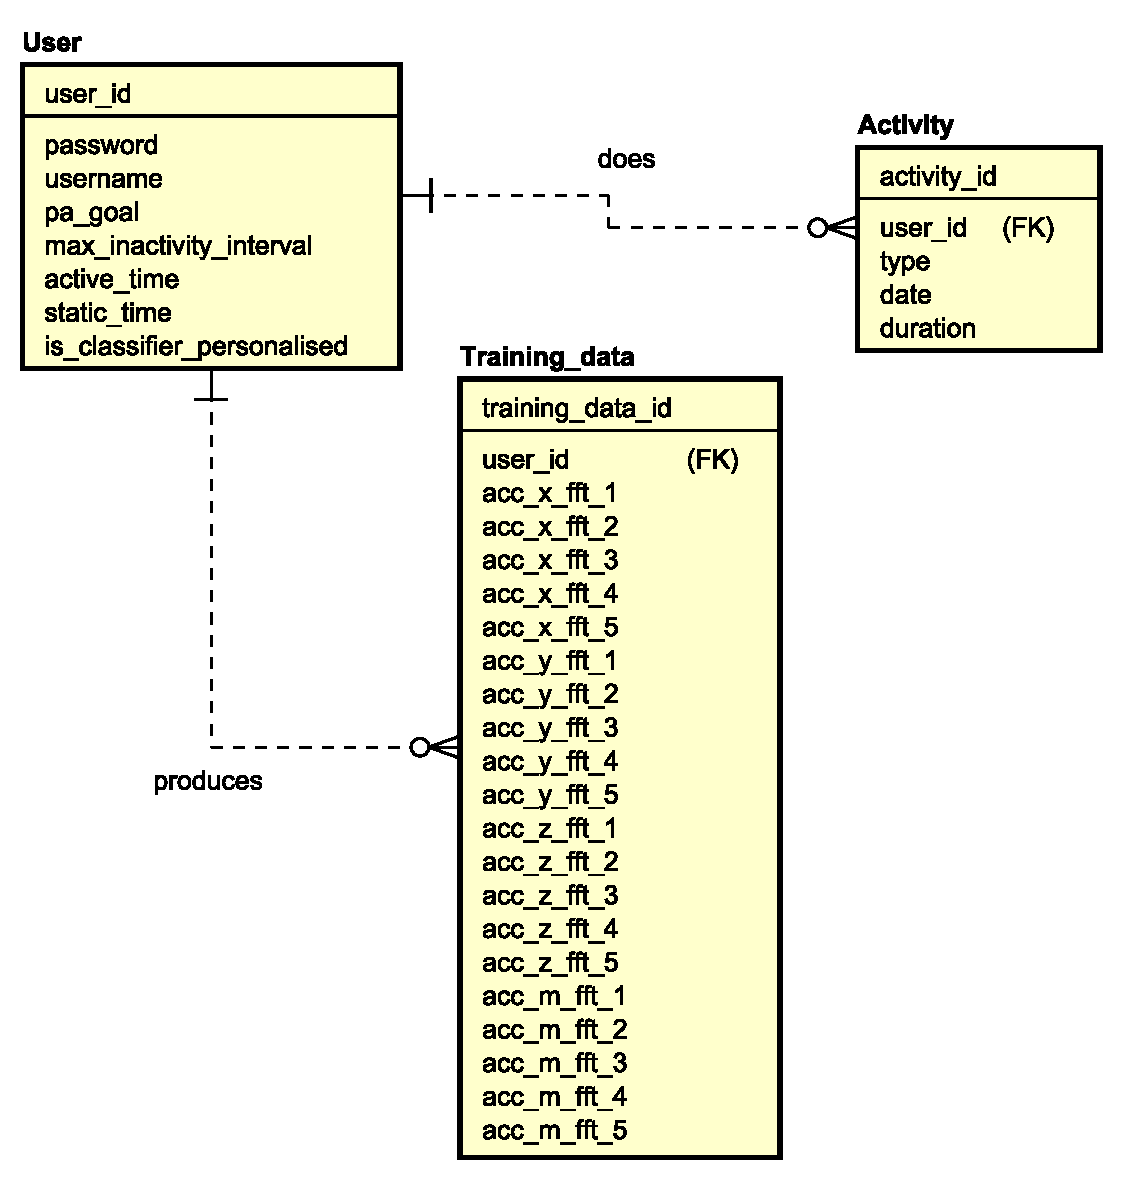
\includegraphics[width=12cm]{data-modeling-er-diagram}
            \caption{Database ER Diagram}
            \label{fig:data_modeling_er_diagram}
        \end{figure}
        
        \subsubsection{Entities}
        
        \begin{itemize}
            \item User(user\_id, password, username, pa\_goal,max\_inactivity\_time)
            \item Training\_data(user\_id, acc\_x\_fft\_1, acc\_x\_fft\_2, acc\_x\_fft\_3, acc\_x\_fft\_4...)
            \item Activity(activity\_id, user\_id, type, date, duration)
        \end{itemize}
        
        \subsubsection{Relationships}
        \begin{itemize}
        \item Does --- User does Activity [1:m][m:o]
        \item Produces --- User produces Training\_data [1:m][m:o]
        \end{itemize}
        
        \subsection{User}
        The user table is responsible for storing the personal information of every registered user. For example, \textbf{\textit{user\_id}} (number) will allow every user to be uniquely identified so further information can be accessed. The table will also store the \textbf{\textit{username}} and \textbf{\textit{password}} of every user. These fields are used for the authenticating different users of the application upon login.
        
        Also, the user table will store additional information such as the \gls{pa} goal and the maximum sedentary time (both in minutes) before a notification is send to remind the current logged-in user for the prolonged inactivity. Last but not least, the table stores \textbf{\textit{active\_time}} and \textbf{\textit{static\_time}}. These fields track the amount of activity and inactivity in minutes, respectively.  
        
        \subsection{Activity}
        As it can be seen from figure \ref{fig:data_modeling_er_diagram}, the Activity table is responsible for storing information for the different activities. Every activity entry in this table has a unique identifier \textbf{\textit{activity\_id}} so every record is uniquely identified in the table itself. Also, this table has \textbf{\textit{user\_id}} field which allows for associating an activity record with a specific user.
        
        The \textbf{\textit{type}} field of the table is responsible for storing the different types of activities as mentioned in section \ref{subsection:monitoring-component} such as \textit{"walking"} or \textit{"static"}. Field \textbf{\textit{date}} as the name of the field suggest, will store the date when the activity was recorded in time. The last field of the activity table is \textbf{\textit{duration}}, this field stores the duration of the performed activity in seconds.
        
        An example of a table entry:\textit{"5,1,running,2017-01-24 20:16:09,3"}. Where \textit{"5"} is the id of the activity, \textit{"1"} is the id of the user who performed it, the next field is the date and \textit{"3"} is the duration of the activity \textit{running}.
        
        \subsection{Training\_data}
        The last database entity to discus is the Training\_data. The fields from the table \textbf{\textit{acc\_x\_fft\_1}},\newline\textbf{\textit{acc\_x\_fft\_2}},\textbf{\textit{acc\_x\_fft\_3}}... will be responsible for storing the extracted features from the raw accelerometer data as discussed in section \ref{section:proposed-application}. The table field \textbf{\textit{user\_id}} will be used to associate a user with a particular record in the table.
        
        One point to note, this table will be used for two purposes at different times of the development of the project. First, it will be used to store all of the project participants training data. This data will be used to build an initial, general classifier. When a classifier is already build, this table will be used to store the labeled data that will be used to build a personalised classifier for a particular user.
    
    
        
    \section{User Interface Design}
    TO BE DONE